% Autor: Leonhard Segger, Alexander Neuwirth
% Datum: 2017-10-30
\documentclass[
	% Papierformat
	a4paper,
	% Schriftgröße (beliebige Größen mit „fontsize=Xpt“)
	12pt,
	% Schreibt die Papiergröße korrekt ins Ausgabedokument
	pagesize,
	% Sprache für z.B. Babel
	ngerman
]{scrartcl}

% Achtung: Die Reihenfolge der Pakete kann (leider) wichtig sein!
% Insbesondere sollten (so wie hier) babel, fontenc und inputenc (in dieser
% Reihenfolge) als Erstes und hyperref und cleveref (Reihenfolge auch hier
% beachten) als Letztes geladen werden!

% Silbentrennung etc.; Sprache wird durch Option bei \documentclass festgelegt
\usepackage{babel}
% Verwendung der Zeichentabelle T1 (Sonderzeichen etc.)
\usepackage[T1]{fontenc}
% Legt die Zeichenkodierung der Eingabedatei fest, z.B. UTF-8
\usepackage[utf8]{inputenc}
% Schriftart
\usepackage{lmodern}
% Zusätzliche Sonderzeichen
\usepackage{textcomp}

% Mathepaket (intlimits: Grenzen über/unter Integralzeichen)
\usepackage[intlimits]{amsmath}
% Ermöglicht die Nutzung von \SI{Zahl}{Einheit} u.a.
\usepackage{siunitx}
% Zum flexiblen Einbinden von Grafiken (\includegraphics)
\usepackage{graphicx}
% Abbildungen im Fließtext
\usepackage{wrapfig}
% Abbildungen nebeneinander (subfigure, subtable)
\usepackage{subcaption}
% Funktionen für Anführungszeichen
\usepackage{csquotes}
% Zitieren, Bibliographie
\usepackage{biblatex}


% Zur Darstellung von Webadressen
\usepackage{url}
%chemische Formeln
\usepackage[version=4]{mhchem}
% siunitx: Deutsche Ausgabe, Messfehler getrennt mit ± ausgeben
\usepackage{floatrow}
\floatsetup[table]{capposition=top}
% Verlinkt Textstellen im PDF-Dokument
\usepackage[unicode]{hyperref}
% "Schlaue" Referenzen (nach hyperref laden!)
\usepackage{cleveref}
\sisetup{
	locale=DE,
	separate-uncertainty
}
%\bibliography{6Mi_S2_25-10-2017_References}

\begin{document}
	
	\begin{titlepage}
		\centering
		{\scshape\LARGE Versuchsbericht zu \par}
		\vspace{1cm}
		{\scshape\huge M3 - Elaszizität\par}
		\vspace{2.5cm}
		{\LARGE Gruppe 6Mi \par}
		\vspace{0.5cm}
		
		{\large Alexander Neuwirth (E-Mail: a\_neuw01@wwu.de) \par}
		{\large Leonhard Segger (E-Mail: l\_segg03@uni-muenster.de) \par}
		\vfill
		
		durchgeführt am 29.11.2017\par
		betreut von\par
		{\large Christian Thiede}
		
		\vfill
		
		{\large \today\par}
	\end{titlepage}
	\tableofcontents
	\newpage
	
	\section{Kurzfassung}
	***Kurzfassung\\
	Um die Elastizität verschiedener Materialien zu untersuchen, wurden zwei Experimente durchgeführt. Zunächst wurden die Auslenkungen von Stäben unter Last gemessen und daraus deren Elastizität bestimmt. Dies ließ Schlüsse auf die Art der Materialien zu. Dann wurde mithilfe verschiedener angehängter Objekte ein Torsionspendel untersucht und so der Schubmodul des Torsionsdrahtes bestimmt.  %TODO Schubmodul richtig?
	Der so ermittelte Schubmodul wurde mit dem zu erwartenden Wert für das vermutete Material des Drahtes verglichen.

	\section{Methoden}
	***Methoden \\
	*** Paralaxen frei wegen spiegel
	*** Schwing MEsspunkt bei max. Speed
	
	\subsection{Biegung Metallstäbe} %maybe besseren Namen finden
	Zunächst wurde, um den Elastizitätsmodul von verschiedenen Materialien zu bestimmen, ihre Durchbiegung in Abhängigkeit von der auf sie wirkenden Kraft gemessen. Dazu wurden vier Stäbe unterschiedlichen Materials an einem Ende waagerecht eingespannt, an ihr anderes Ende fünf verschiedene Gewichte gehängt und dann die senkrechte Auslenkung dieses Endes gemessen.
	Dabei wurde jeweils zwischen jeder Messung die Ruhelage des Stabes ohne Gewicht neu gemessen. Parallaxenfreiheit beim Ablesen der Auslenkungsskala wurde sichergestellt, indem man so über den Stab gepeilt hat, dass die Reflexion des Stabes im Spiegel hinter dem Stab verschwindet. %hoffe des is verständlich
	Dann wurden die Abmessungen der Stäbe an fünf Stellen je dreimal mit einer Mikrometerschraube  gemessen. Hierdurch wird des Fehler dieser Messung sehr gering, wenn sichergestellt ist, dass kein systematischer Fehler durch eine falsche Nullposition der Mikrometerschraube existiert. Dies wurde sichergestellt, indem die Position der Mikrometerschraube im komplett zugeschraubten Zustand überprüft wurde.
	
	\subsection{Torsionspendel}
	Der zweite Versuch bestand darin die Schwingung eines Torsionspendels zu untersuchen, um den Schubmodul des Drahtes, an dem das Pendel aufgehängt ist zu bestimmen. %TODO Schubmodul richtig?
	 Dazu wurde erst die Schwingungsdauer mit angehängter zylindrischer Scheibe dreimal je über drei Perioden gemessen und der Durchmesser des Torsionsdrahtes an fünf verschiedenen Stellen je drei mal gemessen. Dann wurde noch Höhe, Durchmesser und Masse der Scheibe bestimmt.
	Daraufhin wurde die Schwingung des Torsionspendel mit angehängter Hantel untersucht. Hierzu wurde zunächst die Schwingungsdauer der Hantel ohne aufgelegte Scheiben und dann mit zwei Scheiben, die sich in fünf verschiedenen Abständen vom Schwerpunkt der Hantelachse befanden, über drei Perioden gemessen. Die Abmessungen (4 Messungen) und die Masse der Hantel sowie der Scheiben wurde ebenfalls festgestellt. Die Massen waren auf den betreffenden Teilen angegeben.
	Die Länge des Torsionsdrahtes wurde ebenfalls gemessen und in allen Fällen wurde eine Anfangsauslenkung von etwa 180° verwandt. Die Schwingungsdauer wurde jeweils bestimmt, indem mit einer Stoppuhr gemessen wurde, welche Zeit das Pendel für drei Perioden benötigt. Als Anfangs- und Endpunkt der Messung haben wir die Ruhelage der Scheibe gewählt, da sie sich dort näherungsweise mit konstanter Geschwindigkeit bewegt und man somit der Reaktionsfehler minimiert.
	Alternativ hätte man den linken oder rechten Wendepunkt der Bewegung wählen können. An dieser Stelle bewegt sich das Pendel allerdings langsam und der Zeitraum, in dem das Pendel scheinbar stillsteht, ist verhältnismäßig groß, weshalb das Ende der Bewegung kaum exakt zu erkennen ist.
	
	\section{Ergebnisse und Diskussion}

	\subsection{Beobachtung}
	*** linear-> Fit und Algorithmus angeben vgl. Theorie\\
	*** Biegungen in einen Graphen \\
	*** Graphen beschreiben \\
	*** Unsicherheitenrechnung \\

	\subsubsection{Bestimmen der benötigter Größen und deren Unsicherheiten} %TODO Struktur,Texteinbindung, Tabellen-floating
	In \cref{TabelleUnsicherheiten} sind zunächst die Unsicherheiten der verwendete Messinstrumente aufgelistet.

	\begin{table}[h]
	\centering
	\begin{tabular}{ l | c | c | c | c |}
		& Mikroschraube  & Maßband/Biegungsanzeige & Stoppuhranzeige & Reaktionszeit \\ \hline
		u  & $\SI{0,00577}{mm}$ &  $\SI{0,05774}{cm}$ &  $\SI{0,005774}{s}$ &  $\SI{0,11547}{s}$  \\ \hline
	\end{tabular}
	\caption{Unsicherheiten der verwendeten Messinstrumente. Die Wahrscheinlichkeitsdichtefunktionen wurden als rechteckig angenommen.}
		\label{TabelleUnsicherheiten}
	\end{table} %TODO Texteinbindung

	Wir nehmen an, dass sowohl die Stäbe als auch die Gewichte am Torsionspendel exakte Quader bzw. Zylinder sind. Dies ist natürlich nicht exakt gegeben, aber eine genauere Betrachtung würde ein komplexeres Modell erfordern und die Näherung dürfte in diesem Fall recht präzise sein.
	Für die Abmessungen der Stäbe bilden wir einen Mittelwert aus den je $ n=15 $ Messungen. 
	

	\begin{table}[H]
		\centering
		\begin{tabular}{ r | c | c | c | c | c |} 
			& Stab 1, Breite & Stab 1, Höhe  & Stab 2 & Stab 3 &  Stab 4 \\ \hline
			$ \bar{x} $  & $\SI{0,24848}{cm}$ &  $\SI{0,54966}{cm}$ &  $\SI{0,29313}{cm}$ &  $\SI{0,2976}{cm}$ & $\SI{0,2974}{cm}$  \\ \hline
		\end{tabular}
		\caption{Mittelwerte $ \bar{x} $, die sich aus den Messwerten für die Abmessungen der Stäbe ergeben}
		\label{Abmessungen_Stäbe}
	\end{table}
	Für diesen existiert eine Standardunsicherheit und die Unsicherheit der Mikrometerschraube. Diese kombinieren sich gemäß
	\begin{equation*}
		u(\bar{x})=\sqrt{\left( \frac{u_\text{Schraube}}{n}\right) ^2+u_\text{S}(\bar{x})^2}.
	\end{equation*}
	Dabei gilt für die Standardunsicherheit des Mittelwertes
	\begin{equation*}
		u_\text{S}(\bar{x} ) = \sqrt{\frac{\sum_{i=1}^{n} (x_i-\bar{x})^2}{n(n-1)}}.
	\end{equation*}
	In \cref{Stäbe_Abmesungen_Unsicherheiten} sind die sich daraus ergebenden Unsicherheiten dargestellt. %TODO
	
	\begin{table}[H]
		\centering
		\begin{tabular}{ r | c | c | c | c | c |} 
			& Stab 1, Breite & Stab 1, Höhe  & Stab 2 & Stab 3 &  Stab 4 \\ \hline
			$ u_\text{S} $  & $\SI{0,000165}{cm}$ &  $\SI{0,000222}{cm}$ &  $\SI{0,000192}{cm}$ &  $\SI{0,000131}{cm}$ & $\SI{0,000306}{cm}$  \\ \hline
			$ u $ & $\SI{0,000169}{cm}$ & $\SI{0,000225}{cm}$ & $\SI{0,000196}{cm}$ & $\SI{0,000137}{cm}$ & $\SI{0,000308}{cm}$ \\ \hline
		\end{tabular}
		\caption{Unsicherheiten der Mittelwerte der Abmessungen der Stäbe. Soweit nicht anders gekennzeichnet, bezieht sich der Wert auf den Durchmesser des Stabes. $ u_\text{S} $ meint dabei die Standardunsicherheit und $ u $ die Gesamtunsicherheit.}
		\label{Stäbe_Abmesungen_Unsicherheiten}
	\end{table}
	In gleicher Art und Weise lassen sich die Unsicherheiten der Abmessungen des Torsionsdrahtes, der Scheibe, der Hantel und der Hantelscheiben bestimmen. Dabei gilt für den Torsionsdraht die Unsicherheit der Mikrometerschraube und ansonsten die des Maßbandes. Für die Standardunsicherheiten ergibt sich hier jeweils $u_\text{S}=0 $ und für die Gesamtunsicherheiten beim Torsionsdraht $ u=  \SI{0,00004}{\centi \meter}$ und bei Durchmesser sowie Höhe bzw. Länge der Scheibe, Hantel und Hantelscheiben $ u= \SI{0,0144}{\centi \meter}$.
	Die Massen der Gewichte, mit denen wir die Stäbe und den Torsionsdraht belasten, nehmen wir als exakt an.




	
	\begin{table}[H]
		\centering
		\begin{tabular}{ r | c | c |} 
			& & Abmessungen\\ \hline
			Scheibe & Höhe & \SI{1,9}{\centi \meter }\\
			& Durchmesser & \SI{14,65}{\centi \meter }\\ \hline
			Hantel & Länge & \SI{25,1}{\centi \meter }\\
			& Durchmesser & \SI{1,3}{\centi \meter }\\ \hline
			Hantelscheiben & Höhe & \SI{2}{\centi \meter } \\
			& Durchmesser & \SI{5}{\centi \meter }\\ \hline
		\end{tabular}
		\caption{Mittelwerte, der Messwerten für die Abmessungen der Scheibe, Hantel und Hantelscheiben}
		\label{Abmessungen_Scheiben}
	\end{table}
	\subsubsection{Biegung der Stäbe}
	In \cref{BiegungGraph} sind für jeden der Stäbe 5 Messpunkte der Legende entsprechend dargestellt. Der lineare Zusammenhang ist beim Betrachten der Werte bereits erkennbar und außerdem sollte dieser der Theorie zufolge auftreten. Deshalb haben wir einen Fit mit dem \enquote{Scaled Levenberg-Marquardt}-Algorithmus, welcher die Methode der kleinsten Quadrate verwendet, durchgeführt. Die Fit-Funktion sollte wie folgt aussehen:
	\begin{equation}
		f(x)=a*x+b
	\end{equation}
	\begin{figure}[H]
		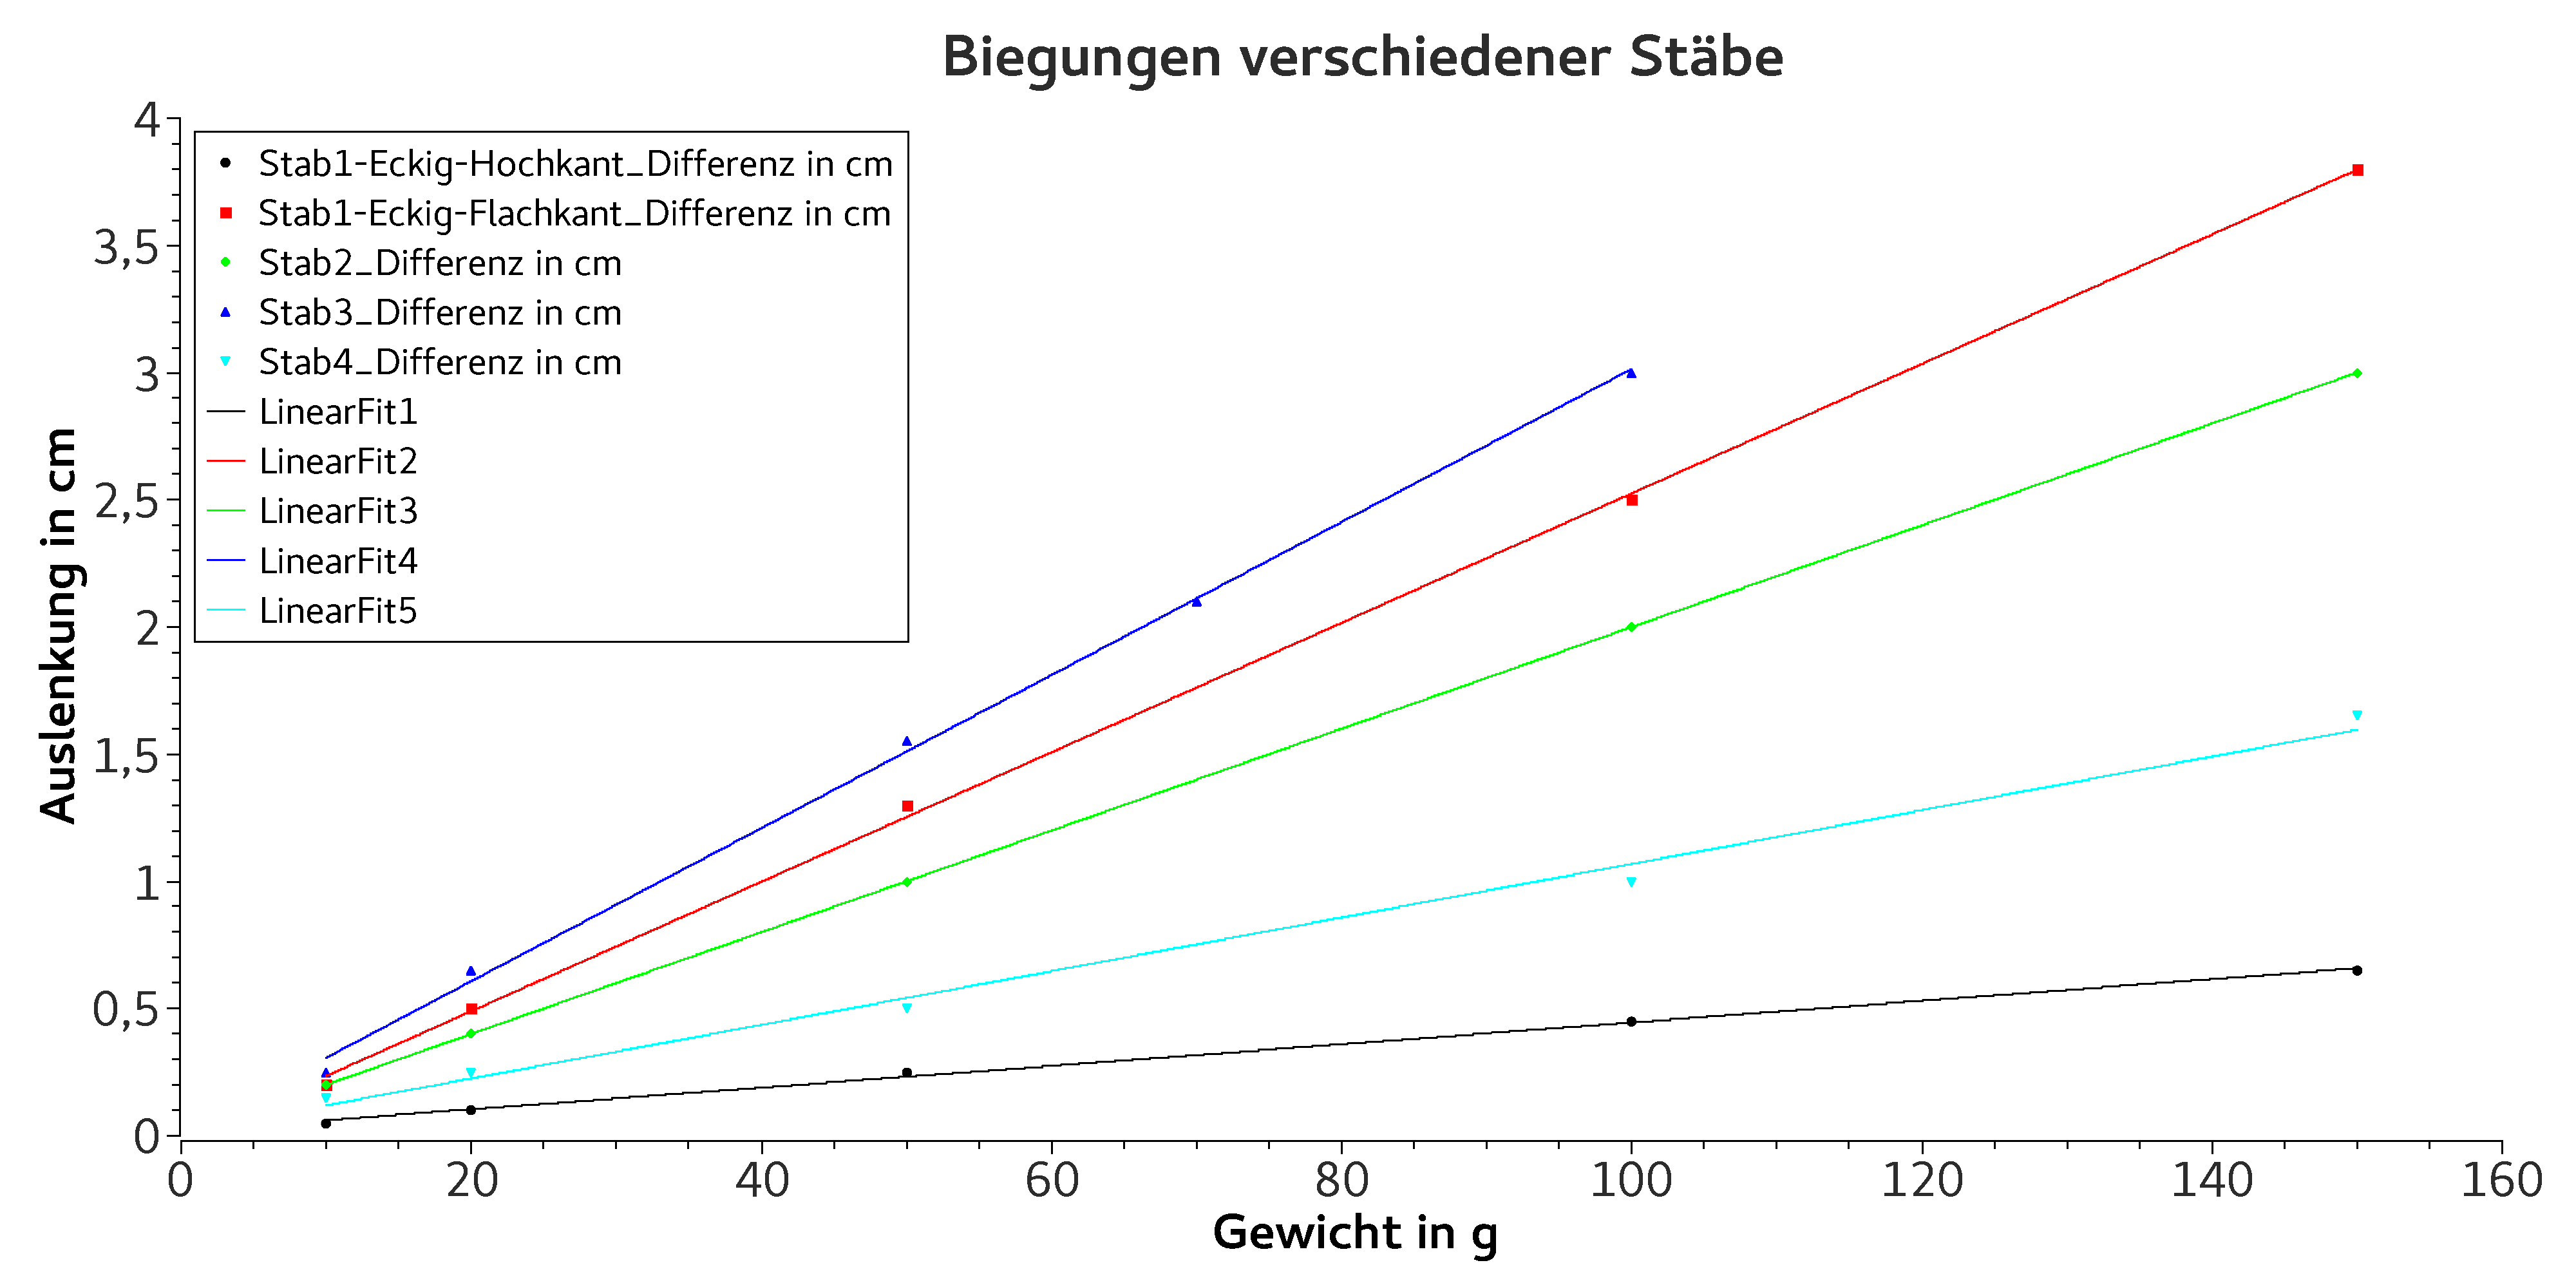
\includegraphics[width=1\textwidth]{Biegungen}
		\centering
		\caption{Biegungen verschiedener Stäbe. Die Fehler sind kleiner als die Symbole}
		\label{BiegungGraph}
		\centering
	\end{figure}

	\begin{table}[H]
	\centering
	\begin{tabular}{ l | c | c | }
		& a in \SI{}{\centi\meter\per\gram} & b in \SI{}{\centi\meter} \\ \hline
		S1 hochkant & $\SI{0,004264 \pm 0,0001}{}$& $\SI{0,018586 \pm 0,01}{}$ \\
		S1 flachkant& $\SI{0,025452 \pm 0,0003}{}$& $\SI{-0,019825 \pm 0,03}{}$ \\ 
		S2 &$ \SI{0,02}{} \pm 6 \cdot 10^{-19}$  &$\SI{0 \pm 5e-17}{}$ \\
		S3 & $\SI{0,030093 \pm 0,0007}{}$ &  $\SI{0,005370 \pm 0,04}{}$\\
		S4 &  $\SI{0,010546 \pm 0,0005}{}$ &$\SI{0,013921 \pm 0,04}{}$  \\ \hline
	\end{tabular}
	\caption{Parameter die sich beim Fitten ergeben}
	\label{TabelleFits}
	\end{table}


	\subsubsection{Torsion des Drahtes}
	In \cref{TorsionGraph} sind für 5 verschiedene Hanteln die Schwingdauerquadrate auf den Radius der Hanteln aufgetragen. Der lineare Zusammenhang ist beim Betrachten der Werte bereits erkennbar und außerdem sollte dieser der Theorie zufolge auftreten. Deshalb haben wir einen Fit mit dem \enquote{Scaled Levenberg-Marquardt}-Algorithmus, welcher die Methode der kleinsten Quadrate verwendet, durchgeführt. Die Fit-Funktion sollte wie folgt aussehen:
	\begin{equation}
		f(x)=A*x+B
	\end{equation}
	\begin{figure}[H]
		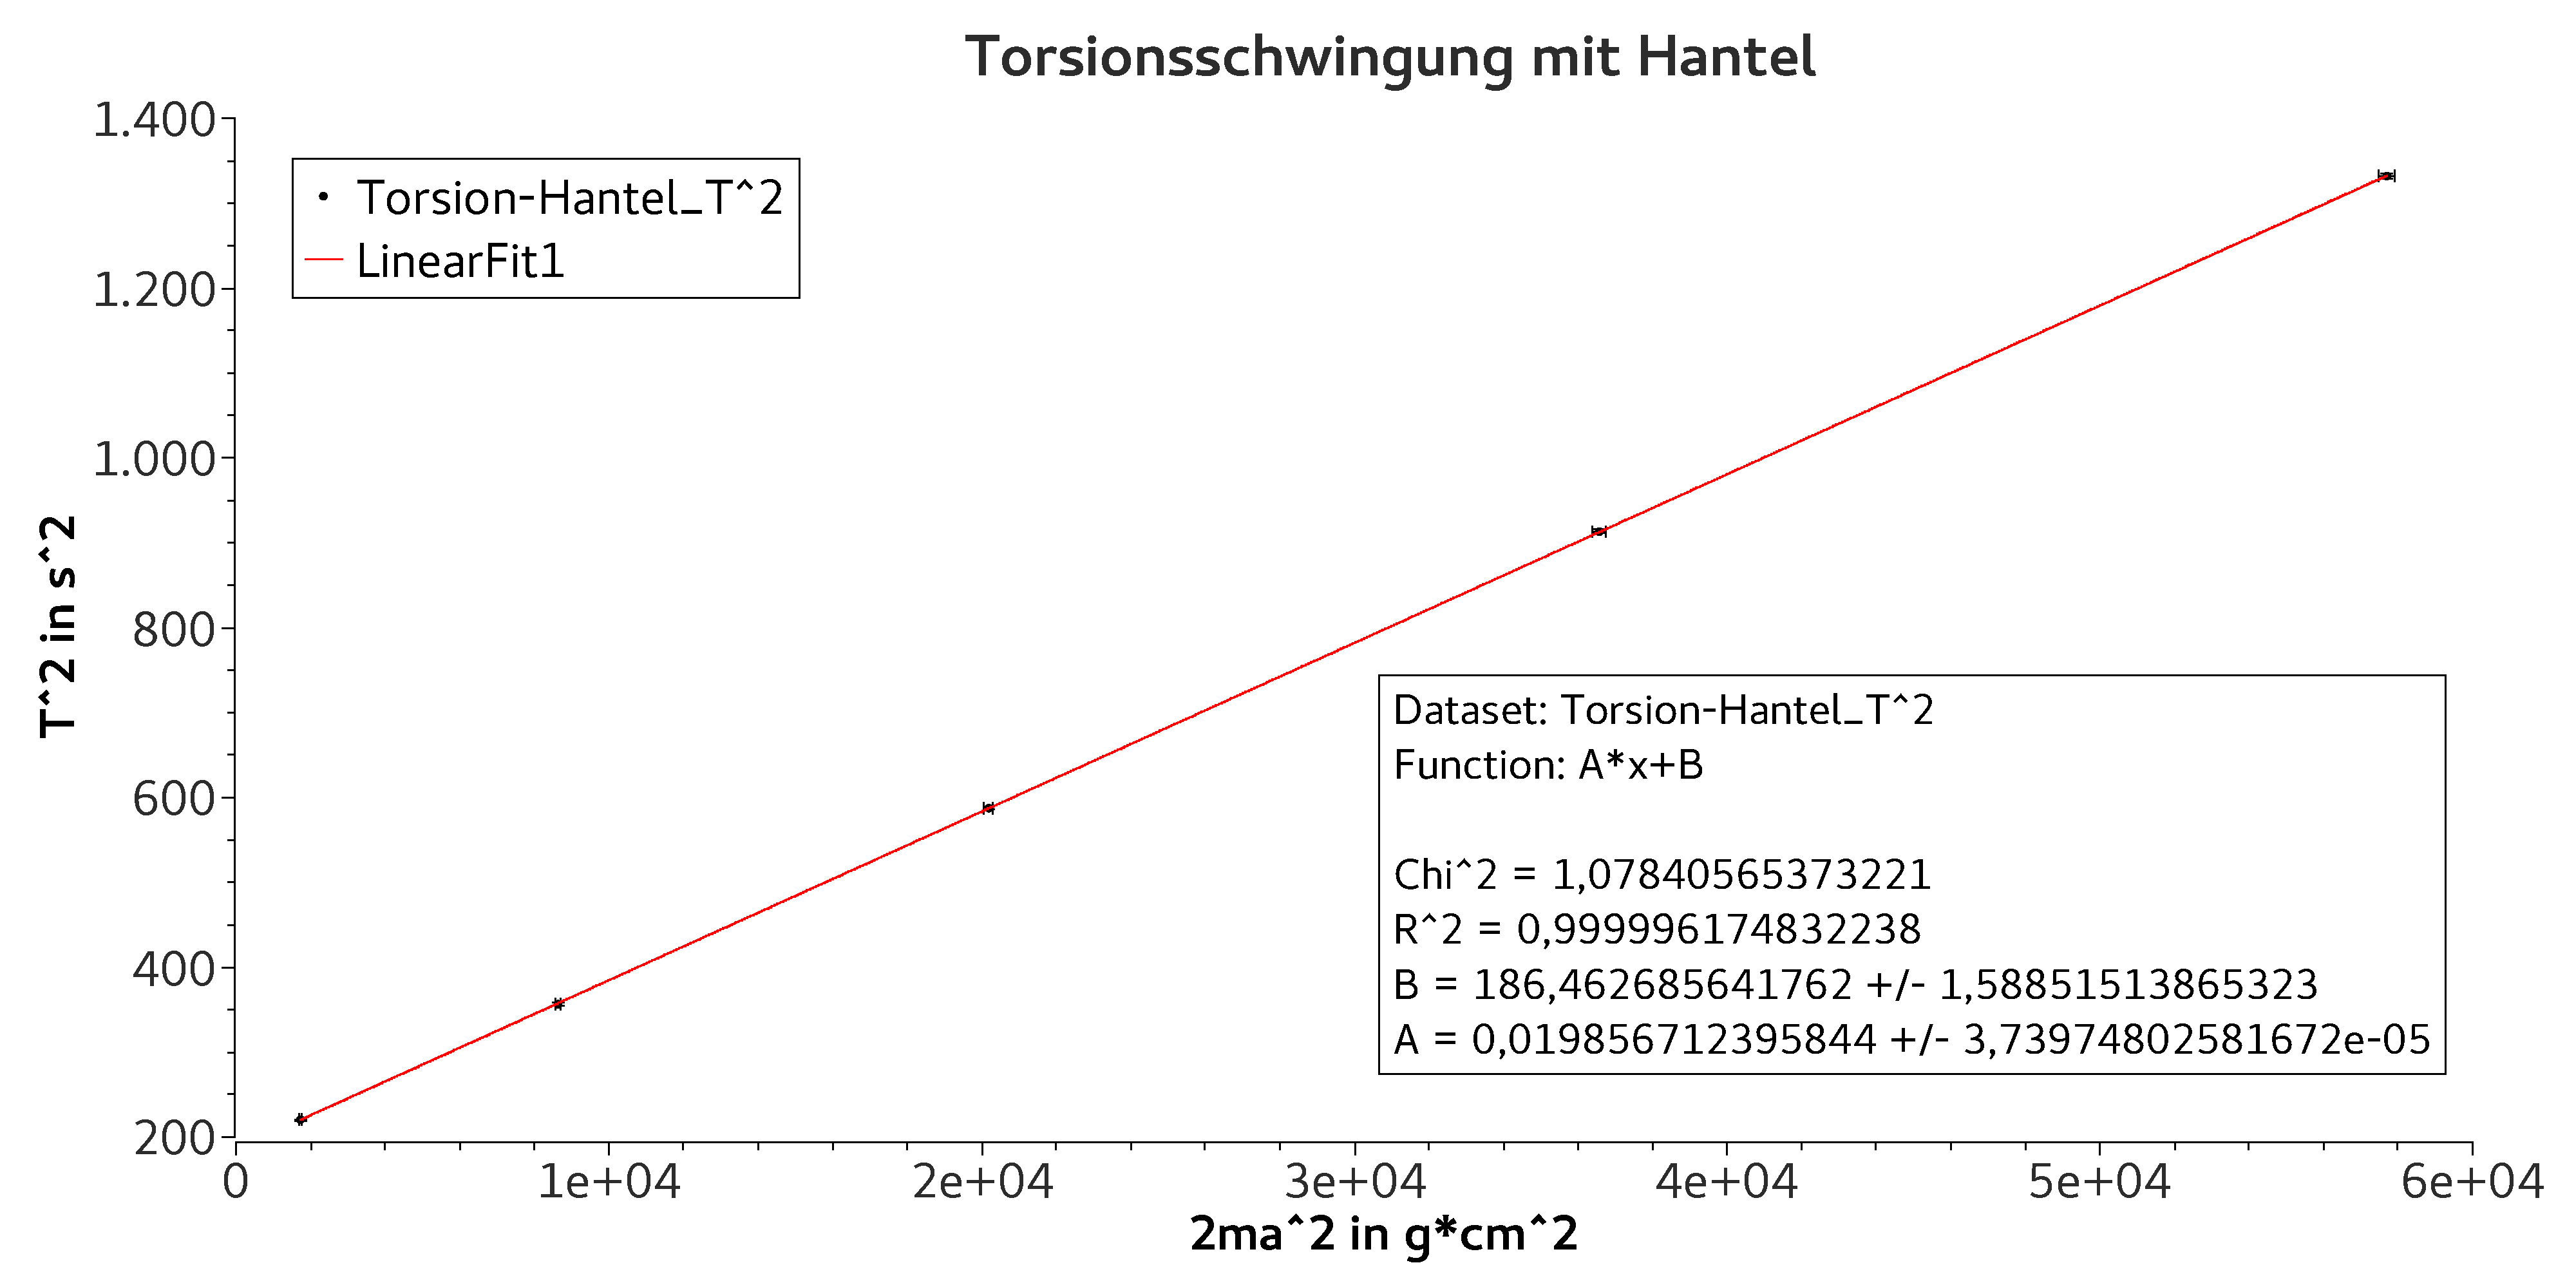
\includegraphics[width=1\textwidth]{Torsion}
		\centering
		\caption{Torsion eines Drahtes mit verschiedene Hanteln. Die Fehler sind kleiner als die Symbole}
		\label{TorsionGraph}
		\centering
	\end{figure}


	
	\subsection{Diskussion}
	*** Gewichte als exakt angenommen
	***Materialien vergleich mit Literatur
	*** kleinste quadrate
	
	\section{Schlussfolgerung}
	***Materialien vergleich mit Literatur \\
	***Das metallene Ende der Maßbänder war lose, was Messung erschwerte.
	
	%\printbibliography
\end{document}
